\chapter{Calcolo Combinatorio}
Per scegliere le strutture combinatorie elementari coinvolte in un problema, occorre rispondere a due domande:
\begin{itemize}[nosep]
    \item l'\textbf{ordine} degli elementi è rilevante oppure no?
    \item gli elementi si possono \textbf{ripetere} oppure no?
\end{itemize}

\section{Strutture Combinatorie Elementari}
\begin{enumerate}[nosep]
    \item una \textbf{disposizione semplice} di $n$ oggetti a $k$ a $k$ con $k \leq n$ è una $k$-upla ordinata di $k$ oggetti distinti scelti tra gli $n$ dati (si tiene conto dell'\textbf{ordine}, \textbf{non} si \textbf{ripetono} gli elementi).
    \begin{boxA}
        Il numero di disposizioni semplici è \fcolorbox{red}{white}{$D(n; k) = n \cdot (n - 1) \cdot ... \cdot (n - k + 1)$} \\
        \textcolor{orange}{\textbf{Esempio}}: In un collegio ci sono 10 professori, in quanti modi possono essere scelti \textit{presidente}, \textit{vicepresidente} e \textit{segretario}
        
        {\centering
            $D_{10, 3} = 10 \cdot 9 \cdot 8$
        \par}
    \end{boxA}
    \item una \textbf{disposizione con ripetizione} di $n$ oggetti a $k$ a $k$ è una $k$-upla ordinata di $k$ (non necessariamente distinti) scelti tra $n$ dati (si tiene conto dell'\textbf{ordine}, si possono \textbf{ripetere} gli elementi).
    \begin{boxA}
        Il numero di disposizioni con ripetizioni di $n$ oggetti a $k$ a $k$ è: \fcolorbox{red}{white}{$D^R(n; k) = n^k$} \\
        \textcolor{orange}{\textbf{Esempio}}: In un collegio ci sono 10 professori, in quanti modi posso scegliere i tutor per i 3 vincitori (un professore può essere tutor di più professori)

        {\centering
            $D^R_{10,3} = 10^3$
        \par}
    \end{boxA}
    
    \newpage
    \item una \textbf{permutazione} di $n$ oggetti è una $n$-upla ordinata i cui elementi sono tutti gli $n$ oggetti (è una disposizione semplice di $n$ oggetti a $n$ a $n$). Il numero di permutazioni di $n$ oggetti è:
    
    {\centering
        \fcolorbox{red}{white}{$P(n) = n!$}
    \par}
    
    \item una \textbf{combinazione semplice} di $n$ oggetti a $k$ a $k$ (con $k \leq n$) è un sottoinsieme di $k$ oggetti distinti scelti tra gli $n$ dati (in questo caso \textbf{non} conta l'\textbf{ordine} e \textbf{non} posso ripetere gli elementi).
    \begin{boxA}
        Il numero di combinazioni semplici di $n$ oggetti a $k$ a $k$ è il ``\textit{coefficiente binomiale}'' di $n$ su $k$: \fcolorbox{red}{white}{$C(n; k) = \binom{n}{k} = \frac{n!}{k! \cdot (n - k)!}$} \\
        \textcolor{orange}{\textbf{Esempio}}: In un collegio di sono 10 professori, in quanti modi posso scegliere 3 professori per la commissione

        {\centering
            $C_{10,3} = \binom{10}{3} = \frac{10!}{3! \cdot (10 - 3)!} = \frac{10!}{3! \cdot 7!} = \frac{10 \cdot 9 \cdot 8 \cdot \cancel{7!}}{3! \cdot \cancel{7!}} = \frac{10 \cdot 9 \cdot 8}{3!}$
        \par}
    \end{boxA}
\end{enumerate}

\begin{flushleft}
    \textbf{Definizione}: un \textbf{Multinsieme} di cardinalità $k$ è una collezione di oggetti, ciascuno ripetuto con una data molteplicità, in modo che la somma delle molteplicità sia pari a $k$. 

    \textbf{Definizione}: una \textbf{combinazione con ripetizione} di $n$ oggetti a $k$ a $k$ è una collezione di $k$ oggetti (non necessariamente distinti) scelti tra gli $n$ oggetti dati (ovvero: è un \textit{sotto-insieme} di cardinalità $k$ dell'insieme di $n$ oggetti dati). Il numero di combinazioni con ripetizioni di $n$ oggetti a $k$ a $k$ è:

    {\centering
        \fcolorbox{red}{white}{$C^R(n; k) = \binom{n + k - 1}{k}$}
    \par}

    \textbf{N.B.}: la differenza tra \textbf{insieme} e \textbf{multinsieme} è che un insieme a tutti gli elementi distinti, mentre un multinsieme ammette anche elementi ripetuti.
    \begin{boxA}
        \textcolor{olive}{\textbf{Dimostrazione}}: consideriamo $\mathbb{N}_n = \{1, 2, ..., n - 1\}$, per avere una combinazione con ripetizione di $k$ elementi in $\mathbb{N}_n$, devo scegliere:

        {\centering
            $1 \leq a_1 \leq a_2 \leq ... \leq a_{k - 1} \leq a_k \leq n$
        \par}
        Osservando le combinazioni semplici, cioè con elementi tutti distinti: \newline
        $1 \leq a_1 < a_2 + 1 \leq a_3 + 1 \leq ... \leq n + 1$ \newline
        $1 \leq a_1 < a_2 + 1 < a_3 + 1 + 1 \leq ... \leq n + 1 + 1$ \newline
        $\cdots$ \newline
        $1 \leq a_1 < a_2 + 1 < a_3 + 2 < ... < a_{k - 1} + (k - 2) < a_k + (k - 1) \leq n + (k - 1)$

        Questo implica che, svegliere $k$ elementi con ripetizione tra $1$ e $n$, è come scegliere $k$ elementi distinti tra $1$ e $n + (k - 1)$, quindi il numero di combinazioni con ripetinizioni di $n$ elementi a $k$ a $k$ è: $C^R(n; k) = C^R(n + k -1; k) = \binom{n + k - 1}{k}$ 
    \end{boxA}
    \begin{boxA}
        \textcolor{orange}{\textbf{Esempi}}
        \begin{enumerate}[nosep]
            \item consideriamo la parola ``discreta'', quanti sono gli anagrammi (anche senza senso). Consideriamo che l'insieme $\mathbb{S} = \{d, i, s, c, r, e, t, a\}$ ogni suo elemento ha \textbf{molteplicità} uno, quindi l'esercizio si risolve con una \textbf{permutazione}:

            {\centering
                $P_3 = 8!$
            \par}
            \item consideriamo la parola ``matematica'', quanti sono gli anagrammi (anche senza senso). Consideriamo l'insieme $\mathbb{S} = \{m, a, t, e, i,c\}$ in questo caso non tutti gli elementi dell'insieme hanno molteplicità uno, ad esempio, $a$ ha molteplicità tre. Quindi dobbiamo utilizzare una \textbf{Permutazione su un multinsieme}.
        \end{enumerate}
    \end{boxA}

    Una \textbf{Permutazione su un Multinsieme} di cardinalità $n$, i cui elementi hanno rispettivamente molteplicità $k_1, ..., k_r$ (con $r \geq 1, \; k_1 \geq 1 \; \forall i \in \{1, ..., r\}$ e tali che $\sum_{i = 1}^r k_i = n$) è una $n$-upla ordinata i cui elementi sono tutti gli $n$ oggetti (non tutti distinti) del multinsieme. Il numero di permutazioni su un multinsieme è pari:

    {\centering
        \fcolorbox{red}{white}{$P^R(n; k_1, k_2, ..., k_r) = \frac{n!}{k_1 \cdot k_2 \cdot ... \cdot k_r}$}
    \par}
\end{flushleft}

\section{Principi Fondanti del Calcolo Combinatorio}

\begin{itemize}[nosep]
    \item \textbf{Principio della Somma}: dati due insiemi finiti e disgiunti $A$ e $B$, allora: \fcolorbox{red}{white}{$\# (A \cup B) = \# A + \# B$}
    \item \textbf{Principio Generalizzato della Somma}: dati $n$ insiemi finiti $A_1, A_2, ..., A_n$ con $A_i \cap A_j = \emptyset \; \forall i \neq j \; i,j \in \mathbb{N}_n$, allora: \fcolorbox{red}{white}{$\# (\underset{i \in \mathbb{N}_n}{\bigcup} A_i) = \underset{i \in \mathbb{N}_n}{\sum}\# A_i$}
    \item \textbf{Principio del Prodotto}: dati due insiemi finiti $A$ e $B$, allora: \fcolorbox{red}{white}{$\# (A \times B) = \# A \cdot \# B$}
    \item \textbf{Principio Generalizzato del Prodotto}: dati $n$ insiemi finiti $A_1, A_2, ..., A_n$ allora: \\
    \fcolorbox{red}{white}{$\# (A_1 \times A_2 \times ... \times A_n) = \underset{i \in \mathbb{N}_n}{\prod} \# A_i$}
    \item \textbf{Principio di Inclusione/Esclusione}: siano $A$ e $B$ insiemi finiti, con $\# A = n$ e $\# B = m$, allora: \fcolorbox{red}{white}{$\# (A \cup B) = \# A + \# B - \# (A \cap B)$}

    \begin{center}
        \begin{minipage}[t]{0.1\textwidth}
            \centering
            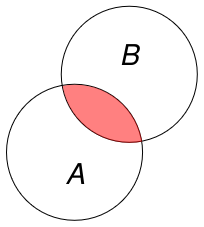
\includegraphics[width=\textwidth]{img/inc_escl_1}
        \end{minipage}
        \hfill
        \begin{minipage}[t]{0.8\textwidth}
            \begin{boxA}
                \textcolor{olive}{\textbf{Dimostrazione}}: consideriamo l'unione disgiunta: $A \cup B = A \cup (B - A)$ \\
                $\Rightarrow \# (A \cup B) = \# A + \fcolorbox{red}{white}{$\# (B - A)$}$, mentre B lo posso vedere come: \\
                $B = (B - A) \cup (A \cap B) \rightarrow \# B = \# (B - A) + \# (A \cap B)$ Quindi avremo \\
                $\fcolorbox{red}{white}{$\# (B - A)$} = \# B - \# (A \cap B)$, sostituendo 
                
                {\centering
                    \fcolorbox{red}{white}{$\# (A \cup B) = \# A + \# B - \# (A \cap B)$}
                \par}
            \end{boxA}
        \end{minipage}
    \end{center}

    \newpage
    \item \textbf{Principio di Inclusione/Esclusione con tre Insiemi}: se $A$, $B$ e $C$ sono insiemi finiti, allora: \fcolorbox{red}{white}{$\# (A \cup B \cup C) = \# A + \# B + \# C - \# (A \cap B) - \# (A \cap C) - \# (B \cap C) + \# (A \cap B \cap C)$}

    \begin{figure}[h]
        \centering
        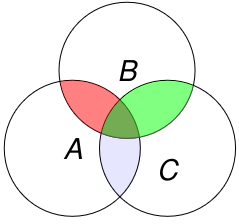
\includegraphics[width=0.1\textwidth]{img/inc_escl_2}
    \end{figure}
    \begin{boxA}
        \textcolor{olive}{\textbf{Dimostrazione}}
        \begin{align*}
            \# (A \cup B \cup C) &= \# [(A \cup B) \cup C] = \# (A \cup B) + \# C - \# [(A \cup B) \cap C] \\
            &= \# (A \cup B) + \# C - \# [(A \cap C) \cup (B \cap C)] \\
            &= \# A + \# B - \# (A \cap B) + \# C - \# (A \cap C) - \# (B \cap C) + \# (A \cap B \cap C) \\
            &= \underline{\# A + \# B + \# C - \# (A \cap B) - \# (A \cap C) - \# (B \cap C) + \# (A \cap B \cap C)}
        \end{align*}
    \end{boxA}
\end{itemize}

\begin{flushleft}
    \textbf{Formula di Da Silva}: Se $A_1, A_2, ..., A_n$ sono insiemi finiti, allora:

    {\centering
        $\# (\underset{i \in \mathbb{N}_n}{\bigcup} A_i) = \underset{I \subseteq \mathbb{N}_n, \; I \neq \emptyset}{\sum} (-1)^{\# I - 1} \cdot \# (\underset{i \in I}{\bigcap} A_i)$
    \par}
    Generalizzando per $n$ insiemi finiti: vengono aggiunte le cardinalità singole, si tolgono quelle a due a due, si aggiungono quelle a tre a tre, si tolgono quelle a quattro a quattro, e via dicendo. In questo modo avremo $2^n - 1$ addendi.
\end{flushleft}